%% ****** Start of file template.aps ****** %
%%
%%
%%   This file is part of the APS files in the REVTeX 4 distribution.
%%   Version 4.0 of REVTeX, August 2001
%%
%%
%%   Copyright (c) 2001 The American Physical Society.
%%
%%   See the REVTeX 4 README file for restrictions and more information.
%%
%
% This is a template for producing manuscripts for use with REVTEX 4.0
% Copy this file to another name and then work on that file.
% That way, you always have this original template file to use.
%
% Group addresses by affiliation; use superscriptaddress for long
% author lists, or if there are many overlapping affiliations.
% For Phys. Rev. appearance, change preprint to twocolumn.
% Choose pra, prb, prc, prd, pre, prl, prstab, or rmp for journal
%  Add 'draft' option to mark overfull boxes with black boxes
%  Add 'showpacs' option to make PACS codes appear
%  Add 'showkeys' option to make keywords appear
\documentclass{revtex4}
%\documentclass[aps,prl,preprint,superscriptaddress]{revtex4}
%\documentclass[aps,prl,twocolumn,groupedaddress]{revtex4}
\usepackage[dvipdf]{graphicx}
%\usepackage{dcolumn}

% You should use BibTeX and apsrev.bst for references
% Choosing a journal automatically selects the correct APS
% BibTeX style file (bst file), so only uncomment the line
% below if necessary.
%\bibliographystyle{apsrev}

\begin{document}

% Use the \preprint command to place your local institutional report
% number in the upper righthand corner of the title page in preprint mode.
% Multiple \preprint commands are allowed.
% Use the 'preprintnumbers' class option to override journal defaults
% to display numbers if necessary
%\preprint{}

%Title of paper
\title{Statistical Tests of the Randomness of Radioactive Decay}

% repeat the \author .. \affiliation  etc. as needed
% \email, \thanks, \homepage, \altaffiliation all apply to the current
% author. Explanatory text should go in the []'s, actual e-mail
% address or url should go in the {}'s for \email and \homepage.
% Please use the appropriate macro foreach each type of information

% \affiliation command applies to all authors since the last
% \affiliation command. The \affiliation command should follow the
% other information
% \affiliation can be followed by \email, \homepage, \thanks as well.
\author{Physics 2501: Mechanics and Electromagnetism Laboratory}
%\homepage[]{Your web page}
%\thanks{}
%\altaffiliation{}
\affiliation{Dept. of Physics, University of Connecticut}
%\author{R.T. Jones}
%\affiliation{University of Connecticut}

%Collaboration name if desired (requires use of superscriptaddress
%option in \documentclass). \noaffiliation is required (may also be
%used with the \author command).
%\collaboration can be followed by \email, \homepage, \thanks as well.
%\collaboration{}
%\noaffiliation

\date{\today}

%\begin{abstract}
% insert abstract here
%\end{abstract}

% insert suggested PACS numbers in braces on next line
%\pacs{}
% insert suggested keywords - APS authors don't need to do this
%\keywords{}

%\setlength{\topmargin}{0in}

%\maketitle must follow title, authors, abstract, \pacs, and \keywords
\maketitle

% body of paper here - Use proper section commands
% References should be done using the \cite, \ref, and \label commands

%% The normal text is displayed in two-column format, but special
%% sections spanning both columns can be inserted within the page
%% format so that long equations can be displayed. Use
%% sparingly.
%%\begin{widetext}
%% put long equation here
%%\end{widetext}
%
%% figures should be put into the text as floats.
%% Use the graphics or graphicx packages (distributed with LaTeX2e)
%% and the \includegraphics macro defined in those packages.
%% See the LaTeX Graphics Companion by Michel Goosens, Sebastian Rahtz,
%% and Frank Mittelbach for instance.
%%
%% Here is an example of the general form of a figure:
%% Fill in the caption in the braces of the \caption{} command. Put the label
%% that you will use with \ref{} command in the braces of the \label{} command.
%% Use the figure* environment if the figure should span across the
%% entire page. There is no need to do explicit centering.
%
%%\begin{turnpage}
%% Surround figure environment with turnpage environment for landscape
%% figure
%% \begin{turnpage}
%% \begin{figure}
%% \includegraphics{}%
%% \caption{\label{}}
%% \end{figure}
%% \end{turnpage}
%
%% tables should appear as floats within the text
%%
%% Here is an example of the general form of a table:
%% Fill in the caption in the braces of the \caption{} command. Put the label
%% that you will use with \ref{} command in the braces of the \label{} command.
%% Insert the column specifiers (l, r, c, d, etc.) in the empty braces of the
%% \begin{tabular}{} command.
%% The ruledtabular enviroment adds doubled rules to table and sets a
%% reasonable default table settings.
%% Use the table* environment to get a full-width table in two-column
%% Add \usepackage{longtable} and the longtable (or longtable*}
%% environment for nicely formatted long tables. Or use the the [H]
%% placement option to break a long table (with less control than 
%% in longtable).
%
%
%% Surround table environment with turnpage environment for landscape
%% table
%% \begin{turnpage}
%% \begin{table}
%% \caption{\label{}}
%% \begin{ruledtabular}
%% \begin{tabular}{}
%% \end{tabular}
%% \end{ruledtabular}
%% \end{table}
%% \end{turnpage}
%
%% Specify following sections are appendices. Use \appendix* if there
%% only one appendix.
%%\appendix
%%\section{}
%

\section{Introduction}

The atom is composed of a massive positively-charged nucleus surrounded by
a cloud of electrons in orbit about it.  Transitions of electrons between
allowed atomic orbitals are what causes atoms to absorb and emit light over
a wide range of wavelengths from the infrared to X-rays.  With the discovery
of radioactivity around the year 1900, it was realized that atoms sometimes
emit radiation at much shorter wavelengths than can be explained by electron
transitions.  Today this is understood to be a consequence of transitions
between allowed levels within the nucleus.  The forces that bind protons
and neutrons together in the nucleus are much stronger than the electromagnetic
force that binds electrons to the atom, so the spacings in potential energy
between allowed nuclear levels are typically much larger than the spacings
between allowed electronic levels.  In spite of the difference in the energy
scale, there are similarities between the transitions that occur between
nuclear states and those that take place between electronic states.  Both
of them conserve energy by emitting or absorbing radiation in quanta whose
energy matches the spacing between two levels; both conserve momentum, so
that an excited atom which emits a photon in a given direction must recoil
in the opposite direction with an impulse equal to the momentum of the
radiated particle(s); and both are governed by the statistics of random
exponential decay.

Whereas electronic transitions almost always involve photons, there is a
greater variety in the different kinds of radiation emitted in radioactive
decay.  Radioactive substances undergo four common types of decay:
alpha ($\alpha$) decay, where the emitted particles are $^4$He nuclei,
beta ($\beta$) decay in which the emitted particles are either electrons or
positrons, gamma ($\gamma$) decay, where the emitted radiation is a high-energy
photon, and fission, where a heavy nucleus splits into two more-or-less equal
lighter nuclei and release energy in the process. In alpha decay the parent
nucleus loses four units of mass and two units of charge, and thus the
resulting daughter atom is of a different element. When a nucleus undergoes
beta decay, the daughter nucleus has the same number of nucleons (mass number)
as the parent but the charge number is incremented or decremented by one.
Emitted simultaneously with the beta particle in beta decay is a light neutral
particle called the neutrino.  The parent nucleus is often left in an
energetically excited state following an alpha or beta decay process,
which then decays to the ground state of the daughter nucleus through a
subsequent gamma decay. Transitions between different nuclear energy levels
of the same isotope are generally accompanied by the emission or absorption
of gamma radiation.  These gamma rays are identical in nature to X-rays,
visible light, radio waves and other forms of electromagnetic radiation,
except that the energies of gamma ray photons are much higher and their
wavelengths are much shorter.

\begin{figure}
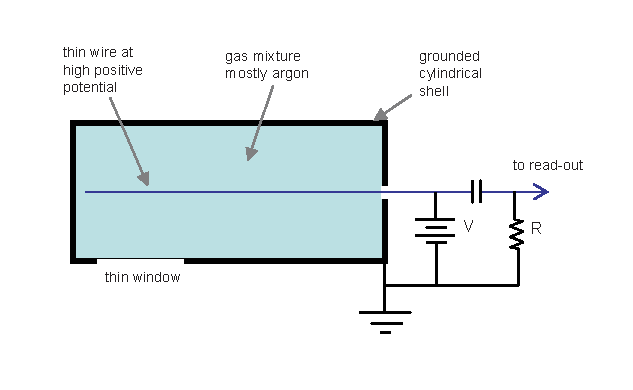
\includegraphics[width=4in]{geigertube.eps}
\caption{\label{geigertube}
Diagram of a Geiger-M\"{u}ller tube, which is used to detect the intensity
of $\beta$ and $\gamma$ radiation by the brief pulse of current that passes
between the electrodes each time atoms in the gas volume are ionized by a
$\beta$ or $\gamma$ particle.  It is insensitive to the alpha particles
from $^{238}$U decay because they cannot travel far enough through the air
to reach the detector, but there are sufficient $\beta$, and $\gamma$
emitters among the secondary nuclei resulting from $^{238}$U decay that a
Geiger counter located several cm away from the source in air has no
difficulty detecting radioactivity from this source.}
\end{figure}

A radioactive decay event is observed when the decay products interact in a
detector.  Most detectors of radioactivity are based on the fact that the
radiation produced by radioactive decay passes through matter and causes
ionization of atoms along its path.  A good example is a Geiger-M\"{u}ller (GM)
tube, which is what you will use in this experiment to detect beta particles
and gamma rays emitted in the decay of $^{238}$U and its daughter nuclei.
The construction of the GM tube is illustrated in Fig.~\ref{geigertube}. The
two electrodes of the GM tube are connected to a high voltage power supply.
Configured in a similar fashion to a cylindrical capacitor, the electric
field inside the tube points radially away from the wire running along its
axis.  When a $\beta$ particle or a $\gamma$ ray passes through the tube, it
can ionize the atoms inside the tube and produce free negatively charged
electrons and positively charged ions. The electrons are accelerated by the
electric field toward the positively charged anode wire.  As dictated by
Gauss' Law, the electric field increases like $1/r$ where $r$ is the distance
from the center of the wire.  As the electrons approach the wire axis, they
pick up kinetic energy at an increasing rate, to the point where they have
enough energy to ionize other atoms in the gas that lie along their path.
This sets up a chain reaction in the strong-field region close to the wire,
resulting in each ionized electron being multiplied into millions of
electrons by the time they reach the wire.  The result is a pulse of
electric charge on the wire that is easily detected and counted by suitable
electronics.  ionization event. This pulse is easily detected and counted by
an electronic counter.

You might wonder why the discharge does not continue forever, turning from
a pulse into a steady electric arc that melts the wire.  The answer lies in
the existence of all of the positive ions that are left behind by the
avalanche of electrons.  These ions are much heavier than the electrons,
and so move much more slowly than the electrons in response to the electric
field.  Instead of being attracted to the positive wire like the electrons
are, they are repelled by the wire.  However they move thousands of times
more slowly because of their large mass, so to the electron pulse they behave
as if they were frozen in place.  This slowly expanding positive cloud of
ions is said to ``screen'' the positive potential of the wire, decreasing
the electric field close to the wire.  One way to think of how this happens
is by the concept of image charges.  Because the wire is a conductor, the
positive ions induce negative image charges inside the wire, which partially
cancel the positive surface charge on the wire electrode.  The net effect is
that the avalanche eventually self-quenches by the build-up of the 
space-charge around the wire.  A related run-away effect called sparking
takes place when the positive ions, which are left in an excited state after
ionization, decay by photon emission, and then those photons are absorbed by
another atom elsewhere in the gas volume, causing ionization and restarting
the avalanche at a different place along the wire.  Sparking is greatly
diminished by the addition of so-called ``quencher'' gases, such isobutane
or ethane, which are strongly absorbing in the UV and have a low probability
for dissipating their excess energy through ionization.  Its simple design,
self-amplifying capability, and its operation with good stability at high
rates, have made the Geiger counter one of the foremost detectors of
radioactivity since it was invented 100 years ago.

\section{Statistical hypothesis of radioactive decay}

One of the enigmas of quantum physics is the randomness of the transitions
that occur between allowed states in a system.  When there are a number of
discrete levels available to a system, according to the theory, the actual
state of the system is not distinct but described by a {\em superposition}
of these levels, each with a complex coefficient called an {\em amplitude}.
The amplitude is sometimes called a {\em wave function} to emphasize the
analogy with the way superposition works in ordinary wave mechanics.  Quantum
mechanics concerns itself with computing these amplitudes, specifically how
they change with time.  In the theory, the amplitudes vary smoothly and
continuously over time.  Suppose the dynamics of the theory predicts a
transition in a nucleus from some excited level $a$ to a lower level $b$.
It does this by making the amplitude for level $a$ gradually decrease
over time, while the amplitude for level $b$ gradually increases.  This is
in stark contrast to what is seen in actual experiments, where a nucleus
is observed to transition abruptly from one level to another by, for example,
the emission of a photon or by $\beta$ decay.

This apparent mismatch between the smooth behavior of amplitudes in the
theory and abrupt transitions in experiment provoked extensive debate
during the formative years of the Quantum Theory, as famously represented
by the Schrodinger's Cat paradox.  Although it remains largely unresolved
to this day, the problem is now considered by most physicists to be a
philosophical one.  Today it goes under the name of {\em the quantum
measurement problem}, which emphasizes the role played by the observer
in the apparent interruption of the smooth time evolution of quantum systems.
For the purposes of this experiment, you should adopt the practical point
of view that the quantum amplitude provides a probability that a given event
will occur within a given time interval.  By observing many transitions of
the same kind, you will evaluate whether your observations are consistent
with a probabilistic interpretation or not.

The radioactive sample you will study in this experiment contains a low
concentration of uranium, mostly $^{238}$U.  According to the table of
the nuclides, Uranium-238 decays by alpha emission with a half-life of
$4.5\times 10^{9}$ years.  If this is correct, a single $^{238}$U nucleus
has 50\% probability of undergoing radioactive decay in $4.5\times 10^9$
years, meaning that the probability of seeing any given nucleus decay during
the few hours of this experiment is utterly negligible.  However it is
possible to observe these decays if a large enough sample of radioactive
material is used.  For example, a sample with $4.5\times 10^9$ $^{238}$U
nuclei in it will produce, on average, one decay every two years.  This
seems like a small rate, except that even a tiny sample of 1~$\mu$g of
$^{238}$U contains more than $2\times 10^{15}$ unstable nuclei, resulting
an average decay rate of about one per minute.  This does not mean that if
you count decays from this sample for one-minute intervals you will get one
every time; sometimes you will observe two, three or even more, and
frequently zero.  If the quantum hypothesis of random transitions applies
to radioactive decays then the probabilities for each of these outcomes is 
given by the Poisson distribution.

The Poisson probability distribution gives the probability of observing a
given number of counts in a fixed time interval. The Poisson distribution
applies only if the counts occur in a random manner and the average count
rate $R$ remains constant during the measurement. The probability of
measuring $n$ counts during a time interval $T$ is
\begin{equation}
P(n) = e^{-RT}\frac{(RT)^n}{n!}
\label{eq:Poisson}
\end{equation}
where the expression $n!$ denotes the factorial of $n$.  The probabilities
$P(n)$ have been normalized to sum to 1 over all $n$.
\begin{equation}
\sum_{n=0}^{\infty}P(n)=1
\end{equation}
The mean and standard deviation of the Poisson distribution are defined in
the usual way.
\begin{equation}
\left< n\right>=\sum_{n=0}^{\infty}nP(n)
\label{eq:mean}
\end{equation}
\begin{equation}
\sigma=\sqrt{\sum_{n=0}^{\infty}(n-\left< n\right>)^2P(n)}
\label{eq:stdev}
\end{equation}
Computing these sums leads the the simple result that
\begin{equation}
\left< n\right> = \sigma^2 = RT
\label{eq:relation2RT}
\end{equation}
The result for the mean is obvious because it was stipulated above that the
average count rate is the constant value $R$.  For large $RT$, the Poisson
distribution of Eq.~\ref{eq:Poisson} is closely approximated by the Gaussian
probability distribution. This is demonstrated using Sterling's approximation,
\begin{equation}
\ln{n!} \simeq n\ln{n}-n+\frac{1}{2}\ln{2\pi n}
\label{eq:Stirlings}
\end{equation}
and the Taylor expansion of $\ln{x}$ around 1
\begin{equation}
\ln{x} = (x-1)-\frac{1}{2}(x-1)^2 + \ldots
\end{equation}
leading to the result
\begin{equation}
P(n)\stackrel{RT\gg 1}{\longrightarrow}
G(n) = \frac{1}{\sqrt{2\pi RT}}
e^{-\frac{(n-RT)^2}{2RT}}
\label{eq:Gaussian}
\end{equation}
For extra credit, prove that Eq.~\ref{eq:Gaussian} follows from
Eq.~\ref{eq:Poisson} in the limit of large $RT$.

\section{Method}

The radioactive source you will use for this experiment is a piece of
glass with a yellowish-green tint that contains traces of uranium.  The
uranium was added in the form of an oxide powder to the mix of sand from
which the glass was formed.  Prior to World War II, decorative tableware
such as bowls and vases made from uranium glass were quite common, desired
for the green luminescence that is visible when viewed in a dimly-lit room.
Controls over the manufacturing of radioactive materials that were put in
place during the Cold War, and also increasing awareness by the public of
the health risks of radioactivity in the living environment, have led to
their virtual disappearance from the marketplace, other than in the trade
of antiques.  The glass you will use in this experiment has an extremely
low radioactivity level.  The University of Connecticut Office of
Environmental Health and Safety oversees the use of all radioactive sources
on campus, and imposes strict controls to minimize the risk of untrained
personnel and students to health effects from exposure to radioactivity
emitted by laboratory sources.

The Geiger counter you will use in this experiment is a hand-held unit
the size of a large calculator, made by the manufacturer Medcom and labeled
``RadAlert'' on the front panel.  These devices consume a lot of power when
in operation, so the batteries are removed when they are not in use.  Make
sure a battery is installed before you attempt to turn use it.
The unit is interfaced to a data acquisition board controlled by a LabView
program that records the number of counts in a time window selected by you.
Start the data acquisition by double-clicking on the LabView icon for this
experiment.  Set the number of repetitions to 20, so that each time you
start a measurement it will acquire counts during twenty consecutive time
intervals, each of duration $T$.  When the data acquisition is complete,
it will then display the measured count.

Note that the value of $T$ that you use in analyzing these data should be
a bit less than the time interval $T_0$ during with the counts were being
accumulated because of the intrinsic ``dead time'' of a GM tube.  Each time
a current pulse occurs on the output of the GM tube, the counting circuit
detects that the wire current has passed above the detection threshold
and a count is registered.  But before the next pulse can be detected, all of
the electrons from the previous pulse must be drained off the wire and
its current allowed to return to zero, or at least below the detection
threshold.  This means that any radioactive decays that occur during this
``dead time'' immediately following a detected pulse cannot be seen.  To
correct for this, the sum of the dead times for all of the detected events
should be subtracted from the total measurement interval in order to get
the value for $T$, which is the effective period of observation in the
measurement.
\begin{equation}
T=T_0(1-Rt_D)
\label{eq:deadtime}
\end{equation}
The typical dead time $t_D$ of a GM tube is of order 1~$\mu$s,
so the effect is not very large at small counting rates, but at rates above
10~kHz the effect can be substantial.

Use Eq.~\ref{eq:relation2RT} to determine the value of $R$ for your setup.  Be
careful not to move things close by your setup on the laboratory bench
during the experiment, especially the source or the detector, during these
measurements.  This is because $R$ depends not only on the radioactive
intensity of the source but also the distance from the source to the detector,
the size and orientation of the detector, and even other objects on the bench
that might serve as scatterers or absorbers of emitted radiation.  If
something is accidentally moved, rather than going back and starting the
experiment from scratch, it is sufficient to repeat the measurement of $R$
that you did at the beginning, and make sure it has not changed significantly.
If it has changed, it may be possible to adjust the geometry slightly so as
to get back to the initial count rate conditions again, within errors.
Even if you believe nothing has changed, it is a good idea to return and
remeasure $R$ after the scan across different values of $T$ described below,
to insure that your conditions were constant throughout the experiment.

To find the error on your measured value of $R$, use Eq.~\ref{eq:stdev} to
estimate the error on each of the values $n_i$ that you obtained, where 
$i=1,\ldots,20$, or more generally $i=1,\ldots,s$ where $s$ is the number
of samplings of the same time interval that you took.  This should be in
approximate agreement with the standard deviation of the numbers $n_i$.
The best estimate for $R$ based on these measurements is the average of
the $n_i$ divided by $T$.  Recall that the error on the average of several
measurements of the same quantity is the error on the individual measurements
divided by $\sqrt{s}$.  Use this result to compute the error on $R$.  You
should increase the counting interval and the repeat count until your 
resulting value of $R$ is accurate to at least two significant digits.

Record results for counting intervals $T$ of 1, 2.5, 5, 10, and 25~s.
Make a log-log plot of the means and variances (square of the standard
deviation) of the $n_i$ as a function of $T$ and fit the data to a straight
line.  Compare the slope of each best-fit line to the value of $R$ you
obtained earlier.  Check that the $y-intercept$ in each case is consistent
with zero.  What do you conclude from the best-fit $\chi^2$ value about the
consistency between the data and the fit?  If you had to chose one of them,
which of the two plots gives a more precise estimate for $R$?  Sometimes
it happens that the more precise estimate is further away from the true
value than a less precise one.  Explain how that is possible.

Place the detector directly on top of the radioactive source, and measure
the count rate.  Now move the sample away until the counting rate decreases
to between 10 and 20 counts per second.  The data you collect next will be
assembled into a frequency table that will be used to test the hypothesis
of randomness in radioactive decay.  A histogram is a special kind of bar
chart that represents a random variable like $n$ on the $x$-axis and the
frequency of observing that value for $n$ on the $y$-axis.  For example, if
you collected 20 observations of 2 minutes each, and observed $n=1$ 15 times
and $n=0$ 5 times then the histogram would consist of a bar chart with one
bar representing each of the allowed values for $n$ (0,1,2,$\ldots$) with
all of the bars at zero height except for $n=0$ which is 5 high and $n=1$
which is 15 high.  If the bars represent raw $n$ values then the $y$-axis
should be labeled ``counts'', but if they have been normalized by dividing
by the total number of trials then the $y$-axis should be labeled ``fraction''.

For your first data set, collect enough data to construct a good histogram
with a value for the time window $T$ that is approximately $2/R$, where $R$
is the average count rate under the present conditions.  A histogram can be
considered ``good'' if it contains sufficient statistics that several bins
have non-zero contents and a least one contains more than 10 entries.
Now run the program a second time, but with a much higher value for the mean
number of events $RT$.  To do this, enter a value for $T$ that is about $15/R$.
Be careful not to disturb the setup because you do not want to change the
value of $R$.   Then run the program a third time with $T=5/R$.  When
you are finished, turn off the Medcom detectors and remove the battery to
conserve battery life.

To see how
the Poisson distribution is the unique prediction of the random decay
hypothesis, consider the following.  Suppose I have an unpredictable source
of events, such as calls coming in to the 911 dispatcher, and I want to
test whether the events are truly random or whether they tend to come in
bunches of two or three together.  The fact that on some particular morning
two calls come in seconds apart does not prove that they are correlated;
to prove correlation, one must rule out the possibility that they just
happened to come close together by chance.  Although it may seem impossible
to rule out one of the other of these two hypotheses, using statistical
methods and systematic observations it is possible to tell whether or not
the random hypothesis is correct.  Suppose that over the course of a year,
records show that a 911 dispatch center has received an average of 8000 calls.
Since I know exactly when each call was received, I can build up a table
of how many calls were received in each 5-minute interval during the year,
of which there are over 100,000.  I make a frequency table listing how many
intervals had 0 calls, how many had 1 call, and so on.  Dividing all of
these frequencies by the total number of 5-minute intervals produces a list of
fractions, called a {\em distribution}, whose values sum up to 1.  If the
process is random then the distribution will match the Poisson distribution
given in Eq.~\ref{eq:Poisson} with $T=5$~minutes.  To be comprehensive, this
test should be repeated with other time intervals of 1 minute, 10 minutes,
30 minutes, 2 hours, and so on.  In each case the distributions will look
different because $T$ is different, but each must agree with
Eq.~\ref{eq:Poisson} for {the same value of $R$}.

Create a histogram of your data showing the frequency at which each count value
$n$ occurs.  Make sure to plot it with a bin width of 1.  Now normalize the area
of the of the histogram to 1 by dividing all of the bin values by the total
number of trials.  The normalized histogram bin heights $y(n)$ can be
interpreted directly as an estimate of the normalized probability distribution
$P(n)$ for observing $n$ events during time interval $T$.  Add error bars
$\Delta y_n$ to your plot showing the error on your estimate of the $y_n$
for each bin.  To discover what these errors should be, go back to the
unnormalized histogram that displays counts versus $n$, and compute an
error on the height in each bin as the square root of the number of counts
in that bin.  Normalize these errors using the same factor that you used
to convert counts per bin into $y_n$, and then add them as errors to your
$y_n$ histogram.  Interpreting this plot as an estimate of $P(n)$, use
Eq.~\ref{eq:mean} to estimate the mean number of counts $\left<n\right>$
for this time interval $T$.  Use propagation of errors from the $y_n$ to
obtain an uncertainty on your extracted value for $\left<n\right>$.

Create a histogram, as described above, for each of the three data sets
you collected above.  Use the extracted value of $\left<n\right>$ from each
histogram to compute three estimates for $R$: $R_2$, $R_{15}$, and $R_5$,
together with their errors $\Delta R_2$, $\Delta R_{15}$, and $\Delta R_5$.
The random hypothesis of radioactive decay predicts that these three $R$
values should be consistent with each other, within errors.

Compare each of the three histograms to the Poisson distribution function
computed using an average of the three values of $R$ found in the previous
step, and the value of $T$ corresponding to each data set.  To facilitate
this comparison, overlay graphs of these distribution functions on your 
histogram plots.  Form a $\chi^2$ for each histogram showing the difference
between the measured $y_n$ and $P(n)$ predicted distribution shapes.  In
your report you should discuss what an unacceptable range would be for
$\chi^2$ in order to rule out the hypothesis of randomness in radioactive
decays.  For the data set with the largest $T$, also compare your results
to the Gaussian distribution given in Eq.~\ref{eq:Gaussian}.  Below what
value of $\left<n\right>$ would you expect the difference between the Poisson 
distribution and its Gaussian approximating to be large enough to make
an observable difference in your $\chi^2$ value?

%\begin{table}
%\caption{\label{displacementfig}
%Nkmg cktetchv cpf dtkfigu, cpf vq uocnngt uvtwevwtgu
%nkmgcvqou cpf pwengk, vjku ukorng oqfgn ikxgu korqtvcpv kpukijv kpvq
%vjgdgjcxkqt qh gxgp vjg oquv eqornkecvgf uauvgou yjgp vjgkt fapcokeu
%ctgiqxgtpgf da uocnn fgrctvwtgu htqo gswknkdtkwo.}
%\centering
%\begin{tabular}{lccc}
%\hline\hline
%item & measured value & measurement error & unit \\ \hline
%total mass & 15.67 & 0.02 & kg \\
%length eyes-tailfin & 14.6 & 0.05 & cm \\
%height belly-dorsal & 3.98 & 0.05 & cm \\
%flash response time & 1.23 & 0.15 & s \\
%total turn time & 1.08 & 0.05 & s \\
%turn radius & 0.72 & 0.15 & cm \\
%maximum turn velocity & 22.1 & 0.5 & m/s \\
%\hline\hline
%\end{tabular}
%\end{table}

\begin{acknowledgments}
This document was updated by Prof. Richard Jones, based on an original
write-up by Prof. Doug Hamilton, with updates by Prof. Ed Eyler (2005).
\end{acknowledgments}

%% Create the reference section using BibTeX:
%\bibliography{revtex4}

%\begin{thebibliography}{9}
%\bibitem{PDG2010}
%Particle Data Group, {\em Review of Particle Physics}, Jour.\ Phys.\ G
%{\bf 37}, no. 7A (2010) p. 1.
%\end{thebibliography}

\end{document}
%%
%% ****** End of file template.aps ******
%
%
